% lint-skip: 未完成ステータス（figure/table caption 未対応，人手チェック時に解消予定）
\documentclass[../../main.tex]{subfiles}
\begin{document}

\begin{flushright}
  \footnotesize\textit{【自動文字起こし・要確認】}
\end{flushright}

[解] 題意から$a, b > 1$である．
図形の$y$軸に関する対称性から，$Q, R$は$y$軸に関して対称な点にある．さらにこの時，$QR \parallel x$軸となることから，$QR$と$x^2+y^2=1$の接点は$A(0, -1)$である．（$(0, 1)$は明らかに不適）

\begin{figure}[htbp]
  \centering
  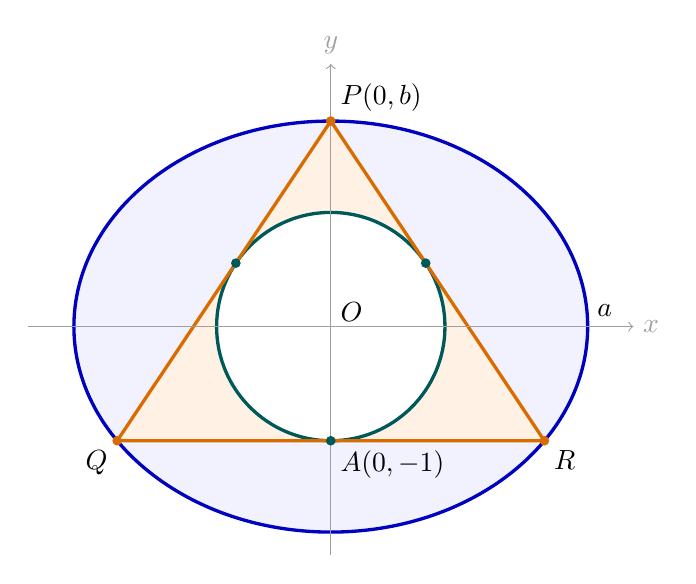
\begin{tikzpicture}[scale=1.45]
    % a=b/(b-1) を満たす例 b=9/5, a=9/4 を作図する。
    \coordinate (O) at (0,0);
    \coordinate (P) at (0,1.8);
    \coordinate (Q) at (-1.8708,-1);
    \coordinate (R) at (1.8708,-1);
    \coordinate (A) at (0,-1);
    \fill[blue!5] (O) ellipse[x radius=2.25,y radius=1.8];
    \draw[blue!75!black,very thick] (O) ellipse[x radius=2.25,y radius=1.8];
    \fill[orange!11] (P)--(Q)--(R)--cycle;
    \fill[white] (O) circle (1);
    \draw[teal!70!black,very thick] (O) circle (1);
    \draw[orange!85!black,very thick] (P)--(Q)--(R)--cycle;
    \draw[->,gray!75] (-2.65,0)--(2.65,0) node[right] {$x$};
    \draw[->,gray!75] (0,-2.0)--(0,2.3) node[above] {$y$};
    \fill[teal!70!black] (-0.8315,0.5556) circle (1.2pt)
    (0.8315,0.5556) circle (1.2pt) (A) circle (1.2pt);
    \fill[orange!85!black] (P) circle (1.2pt)
    (Q) circle (1.2pt) (R) circle (1.2pt);
    \node[above right] at (P) {$P(0,b)$};
    \node[below left] at (Q) {$Q$};
    \node[below right] at (R) {$R$};
    \node[below right] at (A) {$A(0,-1)$};
    \node[above right] at (2.25,0) {$a$};
    \node[right] at (0,0.13) {$O$};
  \end{tikzpicture}
  \caption{楕円と単位円に外接する三角形 $PQR$（図は $b=9/5$）}
\end{figure}

従って，$Q, R$の$y$座標は$-1$です．対称性から $Q\left(-a\sqrt{1-\dfrac{1}{b^2}}, -1\right), R\left(a\sqrt{1-\dfrac{1}{b^2}}, -1\right)$ とおける．以下，$PR$が$x^2+y^2=1$に接する条件をもとめる．（この時，$PQ$も$x^2+y^2=1$と接する）．$\triangle PQR$の面積を2通りで表す．
$$ \dfrac{1}{2}ab\sqrt{1-\dfrac{1}{b^2}} = \dfrac{1}{2}\sqrt{a^2\left(1-\dfrac{1}{b^2}\right) + (1+b)^2} $$
両辺正から2乗して
\begin{align}
  a^2(b^2-1) &= a^2\left(\dfrac{b^2-1}{b^2}\right) + (b+1)^2 \\
  a^2(b^2-1)^2\dfrac{1}{b^2} &= (b+1)^2 \\
  a &= \dfrac{b}{b-1} \quad (a>0, b>1)
\end{align}

\end{document}
